\section{Project Archangel}
Project ARCHANGEL was a decentralized fixity information developed in the UK with the participation of three other countries, Australia, Estonia and Norway. Their approach is to store a cryptographic hash of every incoming object of the archive on a proof-of-authority blockchain. The project started in 2017 and ended in August 2018, the goal of the project was to ensure the integrity and authenticity of digital objects in archives with the usage a private fork of the Ethereum network. Their design philosophy of operating a private blockchain has the flaw of giving a few entities the power to alter data on the blockchain. Currently, their implementation uses smart contracts as a gateway for writing to the Blockchain \cite[4]{collomosse2018archangel}.

The authors of the project ARCHANGEL stated that the trust conferred by the public to the Archives and Memory Institutions (AMIs) had eroded due to the ease by which forgery and unauthorized modifications to electronic records were conducted owing to advances in technology and the generation of numerous types of composited content. To recover public trust in AMIs and guarantee the integrity of the records, a method utilizing the existing databases as well as a method to utilize a merkle tree or  durable storage provided by private corporations have been taken into consideration; however, it was concluded that they are difficult to apply owning to several limitations. Unlike in the past, when archives have relied on the products and technologies of certain companies, blockchain presents a completely different paradigm from openness and expandability. The blockchain awards permission to write records in a distributed ledger to only authorized institutions, whereas permission to view the recorded content after accessing the distributed ledger is granted to every node participating in the blockchain. Moreover, scalability allows the utilization of various tools provided by open-source codes and enables the integrity of records to be assured by multiple parties through a consensus mechanism rather than by a single centralized institution \cite[4]{wang2021research}.

The proposed architecture of ARCHANGEL can be seen in Figure \ref{fig:archangel} where the cryptographic hash of an incoming object is computed and then persisted onto the private blockchain. After a certain time interval, the object can be retrieved from the archived and a hash will be recomputed with the same cryptographic hash function, the object is guaranteed to be unaltered if the local and online hash value are the same.
\begin{figure}[h]
    \caption{Architecture of the ARCHANGEL platform \cite[2]{collomosse2018archangel}}
    \centering
    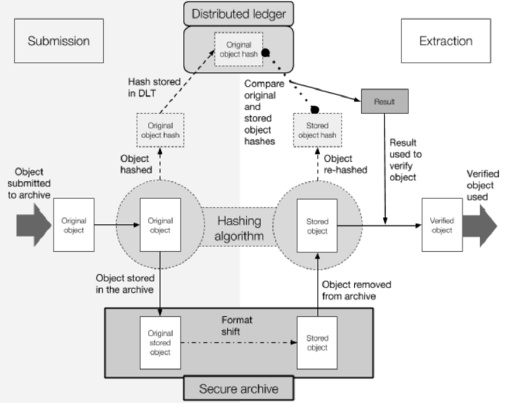
\includegraphics[width=0.5\textwidth]{archangel.png}\label{fig:archangel}
\end{figure}
I agree with their vision of publicly available fixity information, where everyone with an Ethereum client is able to validate the integrity of objects in archive, but there are two points which do not conform with my vision. First and foremost is the usage of a private fork of the Ethereum network that is operated by a private set of nodes, which is basically a proof-of-authority consensus mechanism and contradicts the vision of a decentralized  blockchain \cite[3]{collomosse2018archangel}. Second, they have not implemented some form of transaction reduction, therefore they have to upload a SHA256 word for each object in the archive, which is not feasible since a single upload costs about \$8, see Section \ref{sec:tx-cost}. 

\section{Provenance framework for the IOT}
Sigwart et al. 2020 proposed a generic data provenance framework for the IoT. Their approach is to store provenance records on the Ethereum blockchain with the goal of immutable provenance records for supply chains or sensor data \cite[4]{Sigwart2020}. It is implemented as a framework, therefore it can be adapted to suit other forms of data, in my case fixity information. Their implementation utilized the ERC727 token standard for Ethereum which is beneficial for provenance data, where each object is a non-fungible-token(NFT) \cite[7]{Sigwart2020}. NFTs require a large amount of metadata, which is costly and for my use-case certainly overhead. 

\section{Remote Data Integrity Checking Scheme}
Zhao et al. 2020 proposed a blockchain based remote data integrity checking scheme. Their scheme consists of three phases, including setup, storage and verification phase, this scheme may be of great importance for my work because it integrates well with the work of Sigwart et al. 2020 in terms of design goals. The detail of each phase in their scheme is described as follows: (1) Setup phase, where the public parameter of the elliptic curve group is uploaded to the blockchain. (2) Storage phase, where the data owner signs the data blocks and uploads them to a cloud storage. (3) Verification phase, where the data owner downloads the data or desires to check the integrity of the individual data. The auditing process is done by verifying the signature of the data blocks by the data owner \cite[1]{zhao2020blockchain}.

\section{Pooled testing}\label{sec:pooled}
Pooled Testing was first introduced by \cite{dorfman1943detection} as a strategy to screen numerous military recruits for syphilis during World War 2. Dorfman envisioned that instead of testing each recruit's blood specimen separately, multiple specimens could be pooled together and tested at once. Positive pools' specimens would be retested individually to determine which recruits had contracted the disease, whereas negative pools' specimens would be declared negative. Dorfman wanted to save money on testing while still identifying all syphilitic-positive candidates, so he used group testing. Because the goal is to identify all positive persons among all individuals tested, this is now known as the "case identification problem." Dorfman's case identification method can be thought of as a two-stage hierarchical algorithm. Individuals from positive pools are tested in the second stage after non-overlapping pools have been screened in the first. When the level of corruption is low, higher-stage algorithms have proven to be effective in lowering the number of tests required. \cite[1]{hou2017hierarchical}.
In this thesis, two strategies of pooled testing are implemented. 
First, two stage hierarchical pooling strategy, where in the first stage of this protocol N pools get initialized and filled with samples of the population. If the combined result of the pool is negative than no second stage is needed, but when a pool is declared positive a second stage is needed and all individuals from this pool have to be retested in order to find the corrupted individual. The expected number of test is equal to the number of tests in the first stage added to the number of tests in the second stage \cite[3]{nianogo2021optimal}.
Second, context-sensitive pooling, where homogeneous pool samples are grouped where it is assumed that the within-group variation in any characteristic is smaller than the between-group variation. Hence, if one member of a pooled group is corrupted, there is a high likelihood that other group members are also infected \cite[3]{deckert2020simulation}.

\section{Wrap up}
The blockchain related projects presented in this Chapter have a common vision, which is a decentralized storage for metadata to validate the integrity and authenticity of data used in applications. The ability for the public to validate that an authority did not tamper with the data in their care is important and the removal of trust strengthens the trust in public institutions. More on the subject of trust can be seen in Chapter \ref{ch:diplomatics}
Decentralization and trust aside, the cost of the fixity storage presented in this thesis is also more than relevant as later seen in Chapter \ref{ch:ethereum}, where the cost and computational effort of interacting with the Ethereum network is presented.
